
\section{\BookRecordIndex{T0362}辛微分同胚群}\label{sec:9-5}

本节将证明 Gromov \srcite{160} 关于 $S^2\times S^2$ 与 $\mathbb{CP}^2$ 的\BookRecordIndex{T0362}辛微分同胚
群，以及 $\mathbb R^4$ 的紧支撑辛微分同胚的三个结果。先陈述这些结果。设
$\sigma\in\Omega^2(S^2)$ 是面积为一的标准面积形式，并以
\begin{equation}\label{eq:9-5-1}
  \omega:=\pi_1^*\sigma+\pi_2^*\sigma
  \in\Omega^2(S^2\times S^2)
\end{equation}
表示 $S^2\times S^2$ 上的标准乘积\BookRecordIndex{T0363}辛形式。由于 $S^2\times S^2$ 单连通，其\BookRecordIndex{T0362}辛微分
同胚群的恒等连通分支就是\BookRecordIndex{T0161}哈密顿辛微分同胚群。以下始终把 $S^2$ 与黎曼球面
$\mathbb C\cup\{\infty\}$ 视为同一个空间。

\begin{theorem}[Gromov]\label{thm:9-5-1}
配备\BookRecordIndex{T0363}辛形式~\eqref{eq:9-5-1} 的 $S^2\times S^2$ 之\BookRecordIndex{T0362}辛微分同胚群有两个连通分支。恒等
连通分支同伦等价于 $\operatorname{SO}(3)\times\operatorname{SO}(3)$。
\end{theorem}

\begin{theorem}[Gromov]\label{thm:9-5-2}
设 $V\subset\mathbb R^4$ 是星形紧集，并假设 $0\in\operatorname{int}(V)$。则
$\mathbb R^4$ 的标准\BookRecordIndex{T0363}辛形式 $\omega_0$ 下、支撑在 $V$ 中的辛微分同胚所成群
$\operatorname{Symp}_V(\mathbb R^4,\omega_0)$ 可缩。
\end{theorem}

\begin{theorem}[Gromov]\label{thm:9-5-3}
配备 Fubini--Study 形式 $\omega_{\mathrm{FS}}$ 的 $\mathbb{CP}^2$ 之\BookRecordIndex{T0362}辛微分同胚群同伦
等价于 $\operatorname{PU}(3)$。
\end{theorem}

\begin{remark}\label{rem:9-5-4}
\begin{enumerate}[label=\textup{(\roman*)}]
\item 定理~\ref{thm:9-5-1} 与定理~\ref{thm:9-5-3} 表明：当
$M=\mathbb{CP}^2$，或当 $M=S^2\times S^2$ 且两个因子面积相等时，$M$ 的一个辛微分
同胚光滑同痕于恒等映射，当且仅当它\BookRecordIndex{T0361}辛同痕于恒等映射。Abreu--McDuff \srcite{5} 把
这一结果推广到任意\BookRecordIndex{T0363}辛形式下的 $S^2\times S^2$ 和 $\mathbb{CP}^2$ 的单点吹起。不过，
即便对 $S^2$ 与任意黎曼曲面的乘积，目前也不知道该结论是否对所有\BookRecordIndex{T0363}辛形式成立；它确实在
一个适当的稳定范围内成立，比较 McDuff \srcite{270} 与 Buse \srcite{55}。对一般辛
四维流形，该结论当然不成立。例如，由 Seidel \srcite{368}，余切丛 $T^*S^2$ 的紧支撑
\BookRecordIndex{T0362}辛微分同胚群不具有这个性质。Seidel 在 \srcite{362} 中构造了许多闭辛四维流形的例子，
它们容许光滑同痕于恒等映射、却不\BookRecordIndex{T0361}辛同痕于恒等映射的辛微分同胚。这些例子是沿嵌入
拉格朗日球面 $L\subset M$ 的\BookRecordIndex{T0152}广义 Dehn 扭转 $\tau_L$ 的平方。证明在多数情形
$\tau_L\circ\tau_L$ 不\BookRecordIndex{T0361}辛同痕于恒等映射要用到 \BookRecordIndex{T0132}弗洛尔同调，超出了本书范围。（更多细节
见注~12.6.1。）乘积 $M=S^2\times S^2$ 是一个值得注意的例外：这里反对角线
$L\subset M$ 是拉格朗日球面，但定理~\ref{thm:9-5-1} 表明，此时辛微分同胚
$\tau_L\circ\tau_L$ \BookRecordIndex{T0361}辛同痕于恒等映射。

Seidel 构造的 $\pi_0(\operatorname{Symp}(M,\omega))$ 中的非平凡元素是\emph{脆弱的}：
稍微扰动形式 $\omega$ 的上同调类后，它们就\BookRecordIndex{T0361}辛同痕于恒等映射。Seidel 在
\srcite{372} 中还阐释了\BookRecordIndex{T0365}辛映射类群
$\pi_0(\operatorname{Symp}(M,\omega))$ 的许多其他思想。支持该群应由\BookRecordIndex{T0152}广义 Dehn 扭转
生成这一想法的证据，见 Auroux--Muñoz--Presas \srcite{29}；亦见 Li--Wu
\srcite{246} 及其中的参考文献。除此之外，人们对
$\pi_0(\operatorname{Symp}(M,\omega))$ 的性质研究得相当少；较早的结果有 Ruan
\srcite{339} 关于 $M$ 是 del Pezzo 曲面或 Fano 三维流形的工作，亦见 Li--Li
\srcite{242}。Evans 最近的论文 \srcite{108} 包含其他结果与参考文献。

\item Gromov 早在 \srcite{160} 中就指出，当 $S^2\times S^2$ 的一个球面大于另一个
时，其\BookRecordIndex{T0362}辛微分同胚群的同伦型会改变。他用一个间接论证说明，在这种情形，\BookRecordIndex{T0362}辛微分同胚群的
基本群中存在无限阶元素。后来发现，这个元素同伦于 Hirzebruch 曲面
$\mathbb P(L_2\oplus\mathbb C)$ 上由旋转纤维诱导的圆周作用所成的环路。（记号见例
~\ref{ex:3-3-6}。）如第~\ref{sec:9-7} 节将见，这构成了 \srcite{254} 中在
$S^2\times S^2\times\mathbb T^2$ 上构造不同痕\BookRecordIndex{T0363}辛形式的基础。它也推动了 Abreu
\srcite{3}、Abreu--McDuff \srcite{5} 与 McDuff \srcite{270} 对直纹曲面之\BookRecordIndex{T0362}辛微分
同胚群结构的大量研究。
\end{enumerate}
\end{remark}

对以 $S^2$ 为底的直纹曲面，每当两个球面大小之比越过一个整数，同伦型就会改变。有理
同伦型现已完全清楚；当这个比值位于区间 $(1,2]$ 时，Anjos \srcite{13} 算出了整数同伦
型。此外，她与 Granja 合作证明 \srcite{14}，在这种情形群 $G$ 具有下列群与群同态之图
的\BookRecordIndex{T0326}推出的同伦型：
\[
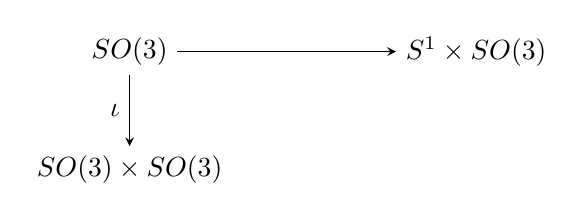
\begin{tikzpicture}[baseline=(current bounding box.center),>=stealth]
  \node (a) at (0,0) {$\operatorname{SO}(3)$};
  \node (b) at (4.4,0) {$S^1\times\operatorname{SO}(3)$};
  \node (c) at (0,-1.5) {$\operatorname{SO}(3)\times\operatorname{SO}(3)$};
  \draw[->] (a) -- (b);
  \draw[->] (a) -- node[left] {$\iota$} (c);
\end{tikzpicture}
\]
竖直同态 $\iota$ 把 $\operatorname{SO}(3)$ 识别为
$\operatorname{SO}(3)\times\operatorname{SO}(3)$ 的对角子群。因此，在同伦理论意义下，
$G$ 是 $\operatorname{SO}(3)\times\operatorname{SO}(3)$ 与
$S^1\times\operatorname{SO}(3)$ 沿 $\operatorname{SO}(3)$ 的\BookRecordIndex{T0068}并合自由积。注意，子群
$S^1\times\operatorname{SO}(3)$ 作为 Hirzebruch 结构 $J_2$ 的自同构群出现在 $G$ 中；
同样，$\operatorname{SO}(3)\times\operatorname{SO}(3)$ 是乘积结构 $J_0$ 的自同构群。
这一思路在 Abreu--Granja--Kitchloo 的论文 \srcite{4} 中达到顶点。

人们或许希望在吹起 $S^2\times S^2$ 的若干点时证明类似结果。Lalonde 和 Pinsonnault
\srcite{229} 在研究单点吹起的\BookRecordIndex{T0362}辛微分同胚群时，发现该群的拓扑与吹起和两个球面的大小
之比之间存在非常有趣的相互作用。另一种观点见 Seidel \srcite{372, Example 1.13}。

现在转入本节开头三个定理的证明。它们的逻辑顺序就是陈述顺序，因为每个定理的证明都
依赖前一个定理。也请注意它与上一节的平行之处。

在证明定理~\ref{thm:9-5-1} 前先引入一些记号。简记
\[
  M:=S^2\times S^2.
\]
由于 $(M,\omega)$ 单调，每个 $\omega$-\BookRecordIndex{T0348}相容\BookRecordIndex{T0088}殆复结构
$J\in\mathcal J:=\mathcal J(M,\omega)$ 都满足命题~\ref{prop:9-4-4} 的假设，即每个
非常值 $J$-全纯球面都有正 Chern 数。以
\[
  A:=[S^2\times\{\mathrm{pt}\}],
  \qquad B:=[\{\mathrm{pt}\}\times S^2]
\]
表示 $H_2(M;\mathbb Z)$ 的标准生成元。令
\[
  \operatorname{Symp}_0:=\operatorname{Symp}_0(M,\omega)
\]
表示在 $H_2(M;\mathbb Z)$ 上诱导恒等映射的辛微分同胚所成群。由于两个球面可以交换，
商群
$\operatorname{Symp}(M,\omega)/\operatorname{Symp}_0(M,\omega)$ 有两个元素。我们需要
证明子群 $\operatorname{Symp}_0(M,\omega)$ 同伦等价于
$\operatorname{SO}(3)\times\operatorname{SO}(3)$。

\begin{proof}[定理~\ref{thm:9-5-1} 的证明]
群 $\operatorname{Symp}_0$ 按
\[
  \operatorname{Symp}_0\times\mathcal J\longrightarrow\mathcal J,
  \qquad(\psi,J)\longmapsto\psi_*J
\]
作用在 $\mathcal J$ 上。乘积复结构 $J_0\in\mathcal J$ 的稳定子是
$\operatorname{SO}(3)\times\operatorname{SO}(3)\subset\operatorname{Symp}_0$。
所以，$\operatorname{Symp}_0$ 在 $J_0$ 上的作用通过
\[
  \operatorname{Symp}_0/
  \bigl(\operatorname{SO}(3)\times\operatorname{SO}(3)\bigr)
  \longrightarrow\mathcal J,
  \qquad\psi\longmapsto\psi_*J_0
\]
把这个商空间与 $J_0$ 的轨道识别起来。该映射显然不是满射；例如，它的像中每个元素都
可积。我们的目标是证明该映射有左逆。

基本思路是：对每个 $J$，指定 $M$ 中通过点 $(0,0)$、分别表示类 $A,B$ 的两个嵌入
$J$-全纯球面。然后还必须为这两条曲线选取参数化。给定两个全纯参数化，正如定理
~\ref{thm:9-4-7}(i) 的证明，可得到微分同胚 $f_J:M\to M$；再用 Moser 同痕以典范方式
把它同痕到一个辛微分同胚。所得辛微分同胚依赖于所选两个 $J$-全纯球面的参数化；模掉
$\operatorname{SO}(3)\times\operatorname{SO}(3)$ 中元素的右乘后，它并非良定义。我们
可以像习题~\ref{ex:7-2-4} 那样选取平衡参数化来绕开这个问题，但从 $\psi_*J_0$ 得到的
陪集未必等于原陪集
$\psi\circ(\operatorname{SO}(3)\times\operatorname{SO}(3))$，尽管二者会以典范方式
同伦。因此，这种做法构造的是同伦左逆。

为了构造严格左逆，注意辛微分同胚 $\psi\in\operatorname{Symp}_0$ 不仅给出\BookRecordIndex{T0088}殆复结构
$J:=\psi_*J_0$，还给出相关两条 \BookRecordIndex{T0003}$J$-全纯曲线的参数化
\[
  z\longmapsto\psi(z,w_*),
  \qquad w\longmapsto\psi(z_*,w),
\]
其中 $\psi(z_*,w_*)=(0,0)$。这提示我们把两条曲线的参数化也纳入参数空间
$\mathcal J$；换言之，考察\BookRecordIndex{T0268}普适模空间
\[
  \mathcal M_0:=\bigl\{(u,v,J)\bigm|
  J\in\mathcal J, u\in\mathcal M(A;J),\ v\in\mathcal M(B;J),
  \ (0,0)\in\operatorname{im}u\cap\operatorname{im}v\bigr\}.
\]
\BookRecordIndex{T0413}重参数化群 $G\times G$ 在这个空间上自由右作用。把命题~\ref{prop:9-4-4} 用于 $p=0$
可知，$(G\times G)$-不变投影 $\mathcal M_0\to\mathcal J$ 是浸没，其纤维就是
$(G\times G)$-轨道。换言之，$\mathcal M_0$ 是结构群为 $G\times G$、底空间为可缩空间
$\mathcal J$ 的主丛。因此它同伦等价于 $G\times G$，进而同伦等价于
$\operatorname{SO}(3)\times\operatorname{SO}(3)$。

考察交换图
\[
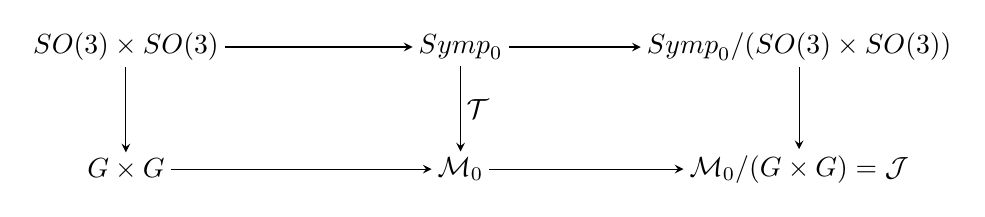
\begin{tikzpicture}[baseline=(current bounding box.center),>=stealth,
  every node/.style={inner sep=2pt}]
  \node (a) at (0,0) {$\operatorname{SO}(3)\times\operatorname{SO}(3)$};
  \node (b) at (4.25,0) {$\operatorname{Symp}_0$};
  \node (c) at (8.55,0)
    {$\operatorname{Symp}_0/(\operatorname{SO}(3)\times\operatorname{SO}(3))$};
  \node (d) at (0,-1.55) {$G\times G$};
  \node (e) at (4.25,-1.55) {$\mathcal M_0$};
  \node (f) at (8.55,-1.55) {$\mathcal M_0/(G\times G)=\mathcal J$};
  \draw[->] (a) -- (b);
  \draw[->] (b) -- (c);
  \draw[->] (d) -- (e);
  \draw[->] (e) -- (f);
  \draw[->] (a) -- (d);
  \draw[->] (b) -- node[right] {$\mathcal T$} (e);
  \draw[->] (c) -- (f);
\end{tikzpicture}
\]
其中嵌入 $\mathcal T:\operatorname{Symp}_0\to\mathcal M_0$ 定义为
\[
  \mathcal T(\psi)
  :=\bigl(\psi(\,·,w_*),\psi(z_*,\,·),\psi_*J_0\bigr),
  \qquad(z_*,w_*):=\psi^{-1}(0,0).
\]
由于 $\mathcal T$ 关于 $\operatorname{SO}(3)\times\operatorname{SO}(3)$ 的右作用等变，
它诱导出从
$\operatorname{Symp}_0/(\operatorname{SO}(3)\times\operatorname{SO}(3))$ 到可缩空间
$\mathcal M_0/(\operatorname{SO}(3)\times\operatorname{SO}(3))$ 的连续映射。因此诱导映射
$\mathcal T:\operatorname{SO}(3)\times\operatorname{SO}(3)\to\mathcal M_0$ 是同伦等价。
而 $\mathcal T$ 在 $\operatorname{SO}(3)\times\operatorname{SO}(3)$ 上单射，其像为
\[
  \mathcal M_{00}:=\bigl\{(u,v,J_0)\bigm|
  u(z)=(\phi(z),0),\ v(w)=(0,\phi'(w)),\
  \phi,\phi'\in\operatorname{SO}(3)\bigr\}.
\]
故存在同伦 $\Psi_t:\mathcal M_0\to\mathcal M_0$（$0\le t\le1$），满足
\[
  \Psi_0(\mathcal M_0)\subset\mathcal M_{00},
  \qquad \Psi_1=\operatorname{id},
  \qquad \Psi_t|_{\mathcal M_{00}}=\operatorname{id}\quad(0\le t\le1).
\]
所以，只要构造 $\mathcal T$ 的左逆
$\mathcal F:\mathcal M_0\to\operatorname{Symp}_0$，复合
\[
  \mathcal F\circ\Psi_t\circ\mathcal T:
  \operatorname{Symp}_0\longrightarrow\operatorname{Symp}_0
\]
就给出所需的变形收缩，把 $\operatorname{Symp}_0$ 收缩到
$\operatorname{SO}(3)\times\operatorname{SO}(3)$。

如下构造 $\mathcal F:\mathcal M_0\to\operatorname{Symp}_0$。三元组
$(u,v,J)\in\mathcal M_0$ 决定两个光滑映射
\[
  S^2\longrightarrow\mathcal M(A;J)/G:w\longmapsto[u_w],
  \qquad
  S^2\longrightarrow\mathcal M(B;J)/G:z\longmapsto[v_z],
\]
使得 $u(z)\in\operatorname{im}[v_z]$ 且
$v(w)\in\operatorname{im}[u_w]$。定义
$\psi=\psi_{u,v,J}:M\to M$ 为
\[
  \psi(z,w):=\operatorname{im}[u_w]\cap\operatorname{im}[v_z].
\]
定理~\ref{thm:9-4-7} 的证明说明，该映射是微分同胚，而且
\begin{equation}\label{eq:9-5-2}
  \psi(z,w_*)=u(z),
  \qquad \psi(z_*,w)=v(w)
\end{equation}
对所有 $z,w\in S^2$ 成立；其中 $z_*,w_*\in S^2$ 选成满足
$u(z_*)=v(w_*)=(0,0)$。该证明还说明，
\[
  \omega_t:=\omega+t(\psi^*\omega-\omega)
\]
对 $0\le t\le1$ 都是\BookRecordIndex{T0363}辛形式。由于 $\psi$ 在 $H^2(M;\mathbb R)$ 上作用为恒等映射，这些
形式彼此上同调。故可用典范 Moser 同痕把 $\psi$ 变形成辛微分同胚：由注
~\ref{rem:9-4-9}，存在只依赖 $\psi$ 的道路 $f_t\in\operatorname{Diff}(M)$，使
$f_0=\operatorname{id}$ 且
\[
  f_1^*\psi^*\omega=\omega.
\]
定义
\[
  \mathcal F(u,v,J):=\psi_{u,v,J}\circ f_1.
\]
注意，只要 $\psi_{u,v,J}$ 本身是辛微分同胚，就有
$\mathcal F(u,v,J)=\psi_{u,v,J}$。所以由式~\eqref{eq:9-5-2}，
$\mathcal F\circ\mathcal T=\operatorname{id}:\operatorname{Symp}_0\to
\operatorname{Symp}_0$，正合所需。定理得证。
\end{proof}


\begin{remark}\label{rem:9-5-5}
定理~\ref{thm:9-5-1} 中，只须证明
$\operatorname{Symp}_0/(\operatorname{SO}(3)\times\operatorname{SO}(3))$ 的所有同伦群
都消失，因为这个商空间具有某个可数 CW 复形的弱同伦型。

这个经典结果似乎没有显然可引的出处，故在此概述论证细节。由 Milnor
\srcite{288, Theorem 1}，只需证明当 $M$ 是闭\BookRecordIndex{T0358}辛流形时，$\operatorname{Symp}(M)$ 具有
\BookRecordIndex{T0206}绝对邻域收缩核（ANR）的同伦型。由 Moser 同痕论证，$\operatorname{Symp}(M)$ 是
$\operatorname{Diff}(M)$ 某个开子集的变形收缩核。因此，只须验证
$\operatorname{Diff}(M)$ 是 ANR。Kriegl--Michor \srcite{218} 指出，
$\operatorname{Diff}(M)$ 自由作用在把 $M$ 光滑嵌入某个固定 Hilbert 空间
$\mathcal H$ 的可缩空间 $\operatorname{Emb}(M,\mathcal H)$ 上。该嵌入空间是 Fréchet
空间的开子集，因而是 ANR。此外，$\operatorname{Diff}(M)$ 是如下投影的纤维：从
$\operatorname{Emb}(M,\mathcal H)$ 投到光滑 Fréchet 流形 $\mathcal M(M)$，后者由
$\mathcal H$ 中所有与 $M$ 微分同胚的嵌入子流形组成。因此，
$\operatorname{Diff}(M)$ 又是 $\operatorname{Emb}(M,\mathcal H)$ 某个开子集的收缩核，
故其自身也是 ANR。
\end{remark}

为了阐明 $S^2\times S^2$ 与 $\mathbb R^4$ 的\BookRecordIndex{T0362}辛微分同胚群之间的关系，考察支撑在闭
双圆盘 $\Delta_r:=D_r\times D_r$ 中的辛微分同胚所成群
$\operatorname{Symp}_{\Delta_r}(\mathbb R^4,\omega_0)$。可把这个群识别为
\[
  \mathcal G_\varepsilon
  :=\bigl\{\psi\in\operatorname{Symp}(S^2\times S^2,\omega)
    \bigm|\psi|_{X_\varepsilon}=\operatorname{id}\bigr\},
\]
其中
\[
  X_\varepsilon:=(S^2\times D_\varepsilon)\cup(D_\varepsilon\times S^2),
  \qquad D_\varepsilon\subset\mathbb C\subset S^2.
\]
$\varepsilon,r$ 的具体取值无关紧要。

\begin{lemma}\label{lem:9-5-6}
当 $r<R$ 时，包含映射
\[
  \operatorname{Symp}_{\Delta_r}(\mathbb R^4,\omega_0)
  \lhook\joinrel\longrightarrow
  \operatorname{Symp}_{\Delta_R}(\mathbb R^4,\omega_0)
\]
零伦。
\sourcefootnote{原书在本引理中把环境写成 $\mathbb R^{2n}$，但此处
$\Delta_r=D_r\times D_r$、与 $S^2\times S^2$ 的紧化以及紧随其后的整个证明都只针对
$\mathbb R^4$；故把环境唯一补正为 $\mathbb R^4$。}
\end{lemma}

\begin{proof}
需要证明，对 $\delta<\varepsilon$，包含
$\mathcal G_\varepsilon\hookrightarrow\mathcal G_\delta$ 同伦于常值映射。考察
\[
  \mathcal J_\varepsilon
  :=\bigl\{J\in\mathcal J(S^2\times S^2,\omega)
  \bigm|J|_{X_\varepsilon}=J_0\bigr\}.
\]
我们将构造光滑映射
$\mathcal F:\mathcal J_\varepsilon\to\mathcal G_\delta$，使对每个
$\psi\in\mathcal G_\varepsilon$ 都有
$\mathcal F(\psi_*J_0)=\psi$。结论便由 $\mathcal J_\varepsilon$ 可缩\BookRecordIndex{T0326}推出。

为构造 $\mathcal F$，采用定理~\ref{thm:9-4-7}(ii) 证明中的论证。在当前情形，
$X_\varepsilon$ 是
$(S^2\times\{0\})\cup(\{0\}\times S^2)$ 的邻域，故取 $z_*=w_*=0$，并定义
\[
  u_*(z)=(z,0),
  \qquad v_*(w)=(0,w).
\]
对每个 $J\in\mathcal J_\varepsilon$，如前定义
$\psi_J\in\operatorname{Diff}(S^2\times S^2)$。于是
\[
  \psi_J(z,w)=\operatorname{im}u_w\cap\operatorname{im}v_z,
\]
其中 $[u_w]\in\mathcal M(A;J)$ 由 $(0,w)\in\operatorname{im}u_w$ 确定，
$[v_z]\in\mathcal M(B;J)$ 由 $(z,0)\in\operatorname{im}v_z$ 确定。该映射形如
\[
  \psi_J(z,w)=
  \begin{cases}
    (z,\phi_2(z,w)),&z\in D_\varepsilon,\\
    (\phi_1(z,w),w),&w\in D_\varepsilon,
  \end{cases}
\]
其中对所有 $z,w\in S^2$，$\phi_1(z,0)=z$ 且 $\phi_2(0,w)=w$。为使该映射在
$X_\delta$ 上为恒等映射，一劳永逸地选定光滑映射 $\rho:S^2\to S^2$，满足
\[
  \rho(z)=z\quad(z\notin D_\varepsilon),
  \qquad \rho=0\quad\text{在 $D_\delta$ 的一个邻域中},
  \qquad \det(d\rho(z))\ge0.
\]
定义 $\psi'_J:M\to M$：在 $M\setminus X_\varepsilon$ 上令
$\psi'_J:=\psi_J$，而在 $X_\varepsilon$ 上令
\[
  \psi'_J(z,w):=
  \begin{cases}
    (z,\phi_2(\rho(z),w)),&z\in D_\varepsilon,\\
    (\phi_1(z,\rho(w)),w),&w\in D_\varepsilon.
  \end{cases}
\]
如前，$\psi'_J=\operatorname{id}$ 在 $X_\delta$ 的一个邻域中成立；而对所有
$z,w\in S^2$，子流形 $\{z\}\times S^2$ 与 $S^2\times\{w\}$ 相对于
$(\psi'_J)^*\omega$ 都是辛的。因此
\[
  \omega\wedge(\psi'_J)^*\omega>0
\]
（习题~\ref{ex:9-4-8}），从而可使用 Moser 同痕。具体而言，满足
\[
  d^*\beta_J=0,
  \qquad d\beta_J=(\psi'_J)^*\omega-\omega
\]
的 $1$-形式 $\beta_J$ 在 $X_\delta$ 的一个邻域中正合，故可按典范方式修改为在
$X_\delta$ 上消失。于是得到只依赖 $\psi'_J$ 的微分同胚 $f_J:M\to M$，满足
\[
  f_J^*(\psi'_J)^*\omega=\omega,
  \qquad f_J|_{X_\delta}=\operatorname{id}.
\]
现在定义
\[
  \mathcal F:\mathcal J_\varepsilon\longrightarrow\mathcal G_\delta,
  \qquad \mathcal F(J):=\psi'_J\circ f_J.
\]
对每个 $\psi\in\mathcal G_\varepsilon$，它满足
$\mathcal F(\psi_*J_0)=\psi$。事实上，若 $J=\psi_*J_0$，则
$\psi_J=\psi$ 在 $X_\varepsilon$ 上是恒等映射，故
$\psi'_J=\psi_J$ 且 $f_J=\operatorname{id}$。引理得证。
\end{proof}

\begin{proof}[定理~\ref{thm:9-5-2} 的证明]
结论由引理~\ref{lem:9-5-6} \BookRecordIndex{T0326}推出。选取实数 $r>0$ 与 $T>1$，使
\[
  \frac1T V\subset\Delta_r\subset\operatorname{int}(V),
\]
并对 $1\le t\le T$ 考察映射族
\[
  \mathcal F_t:\operatorname{Symp}_V(\mathbb R^4,\omega_0)
  \longrightarrow\operatorname{Symp}_V(\mathbb R^4,\omega_0),
  \qquad \mathcal F_t(\phi)(x):=\frac1t\phi(tx).
\]
对每个 $\phi\in\operatorname{Symp}_V(\mathbb R^4,\omega_0)$ 有
$\mathcal F_1(\phi)=\phi$；对所有 $t$ 有
$\mathcal F_t(\operatorname{id})=\operatorname{id}$；并且
\[
  \mathcal F_T\bigl(\operatorname{Symp}_V(\mathbb R^4,\omega_0)\bigr)
  \subset\operatorname{Symp}_{\Delta_r}(\mathbb R^4,\omega_0).
\]
\sourcefootnote{原书在这一个包含式的左端把标准形式下标漏掉，写成了
$\operatorname{Symp}_V(\mathbb R^4,\omega)$；本证明始终固定的是
$\omega_0$，而缩放公式也保持 $\omega_0$，故补上该下标。}
由引理~\ref{lem:9-5-6}，包含
$\operatorname{Symp}_{\Delta_r}(\mathbb R^4,\omega_0)
\hookrightarrow\operatorname{Symp}_V(\mathbb R^4,\omega_0)$ 零伦。因此可把
$\mathcal F_t$ 延拓为区间 $1\le t\le T+1$ 上的同伦，使对每个
$\psi\in\operatorname{Symp}_V(\mathbb R^4,\omega_0)$ 都有
$\mathcal F_{T+1}(\psi)=\operatorname{id}$。所以该群可缩。定理得证。
\end{proof}
\begin{proof}[定理~\ref{thm:9-5-3} 的证明]
为突出主要思想，先证明 $\mathbb{CP}^2$ 的\BookRecordIndex{T0362}辛微分同胚群连通。以
$A:=[\mathbb{CP}^1]\in H_2(\mathbb{CP}^2;\mathbb Z)$ 表示标准生成元，以
$\omega_{\mathrm{FS}}\in\Omega^2(\mathbb{CP}^2)$ 表示满足
$\omega_{\mathrm{FS}}(A)=\pi$ 的 Fubini--Study 形式，并以
$J_0\in\mathcal J:=\mathcal J(\mathbb{CP}^2,\omega_{\mathrm{FS}})$ 表示标准复结构。

给定 $\psi\in\operatorname{Symp}(\mathbb{CP}^2,\omega_{\mathrm{FS}})$，选取从 $J_0$ 到
$J_1=\psi_*J_0$ 的\BookRecordIndex{T0088}殆复结构光滑同伦
$[0,1]\to\mathcal J:t\mapsto J_t$。
\sourcefootnote{原书把终点印作 $J_1=\psi_*J$，但此处只给定了初始标准结构 $J_0$，并且
随后要求 $u_1=\psi\circ u_0$；唯一\BookRecordIndex{T0348}相容的终点是 $\psi_*J_0$。}
由推论~\ref{cor:9-4-5}，存在一族光滑依赖于 $t$、模重参数化唯一的 $J_t$-全纯球面
$u_t\in\mathcal M(A;J_t)$，满足
\[
  u_t(0)=[1:0:0],
  \qquad u_t(\infty)=[0:1:0],
  \qquad u_0(z)=[1:z:0],
  \qquad u_1=\psi\circ u_0.
\]
\sourcefootnote{原书同时固定所有 $u_t$ 的两个\BookRecordIndex{T0066}标记点之像，并要求
$u_1=\psi\circ u_0$；但一般的 $\psi$ 不固定 $[1:0:0]$ 与 $[0:1:0]$，故这些条件并不
\BookRecordIndex{T0348}相容。一种可能的补法是让\BookRecordIndex{T0066}标记点之像随 $t$ 移动，但原书未指定具体选择。后续实际需要的
是连接 $u_0$ 与 $\psi\circ u_0$ 的带\BookRecordIndex{T0067}标架曲线族，因而论证意图仍可辨认。}
这里把 $S^2\cong\mathbb C\cup\{\infty\}$。由于 $S^2$ 单连通，存在辛向量丛同构的光滑
同伦
\[
  \Psi_t:(u_0^*T\mathbb{CP}^2,J_0,\omega_{\mathrm{FS}})
  \longrightarrow(u_t^*T\mathbb{CP}^2,J_t,\omega_{\mathrm{FS}}),
\]
从 $\Psi_0:=\operatorname{id}$ 连到 $\Psi_1:=d\psi(u_0)$，并在如下意义下与 $du_t$ \BookRecordIndex{T0348}相容：
\begin{equation}\label{eq:9-5-3}
  \Psi_0=\operatorname{id},
  \qquad \Psi_tdu_0=du_t,
  \qquad \Psi_tJ_0=J_t\Psi_t,
  \qquad \Psi_t^*\omega_{\mathrm{FS}}=\omega_{\mathrm{FS}}.
\end{equation}
称三元组 $\{J_t,u_t,\Psi_t\}_{0\le t\le1}$ 为 \BookRecordIndex{T0003}$J$-全纯曲线的\emph{\BookRecordIndex{T0085}带标架同痕}。
我们希望构造\BookRecordIndex{T0361}辛同痕
\[
  [0,1]\longrightarrow\operatorname{Symp}(\mathbb{CP}^2,\omega_{\mathrm{FS}}),
  \qquad t\longmapsto\psi_t,
\]
从 $\psi_0=\operatorname{id}$ 连到 $\psi_1=\psi$，并使
\begin{equation}\label{eq:9-5-4}
  \psi_t\circ u_0=u_t,
  \qquad d\psi_t(u_0)=\Psi_t.
\end{equation}
按通常方式，寻找由一族哈密顿函数 $H_t$ 生成的同痕：
\begin{equation}\label{eq:9-5-5}
  \frac d{dt}\psi_t=X_t\circ\psi_t,
  \qquad \iota(X_t)\omega_{\mathrm{FS}}=dH_t.
\end{equation}
回忆，$H_t$ 的辛梯度 $X_t$ 与它相对于度量
$\omega_{\mathrm{FS}}(\,·,J_t\,·)$ 的梯度之间满足
$\operatorname{grad}H_t=J_tX_t$。

式~\eqref{eq:9-5-4} 的第一个条件转化为
\[
  X_t(u_t(z))=\partial_t\psi_t(u_0(z))=\partial_tu_t(z),
  \qquad z\in S^2.
\]
为满足第二个条件，还必须控制 $X_t$ 沿曲线 $\operatorname{im}u_t$ 法方向的导数。事实上，
对每个 $v\in T_{u_0(z)}\mathbb{CP}^2$，需要
\[
\begin{aligned}
  \nabla_t(\Psi_t(z)v)
  &=\nabla_t(d\psi_t(u_0(z))v)\\
  &=\nabla_{d\psi_t(u_0(z))v}X_t(\psi_t(u_0(z)))\\
  &=\nabla_{\Psi_t(z)v}X_t(u_t(z)).
\end{aligned}
\]
这里 $\nabla$ 表示度量 $\omega_{\mathrm{FS}}(\,·,J_t\,·)$ 的 \BookRecordIndex{T0034}Levi--Civita 联络
\sourcefootnote{原书此处写作 $\omega(\,\cdot,J_t\,\cdot)$，但本段的靶流形是
$\mathbb{CP}^2$，其固定\BookRecordIndex{T0363}辛形式为 $\omega_{\mathrm{FS}}$；本节此前的裸记号 $\omega$
专指 $S^2\times S^2$ 上的乘积形式，故补全下标。}，$\nabla_t$
表示相对于时间的协变微分。用 $\operatorname{grad}H_t=J_tX_t$ 表示后，这些条件成为
\begin{equation}\label{eq:9-5-6}
  \begin{aligned}
    \operatorname{grad}H_t(u_t)&=J_t(u_t)\partial_tu_t,\\
    \nabla_{\Psi_tv}(\operatorname{grad}H_t)
      &=J_t\nabla_t(\Psi_tv)
        +(\nabla_{\Psi_t(v)}J_t)\partial_tu_t,
        \qquad v\in u_0^*T\mathbb{CP}^2.
  \end{aligned}
\end{equation}
由于 $\Psi_tdu_0=du_t$，当 $v\in\operatorname{im}du_0(z)$ 时第二个方程归结为第一个。
所以这些条件彼此\BookRecordIndex{T0348}相容，并存在解 $H_t$。

现令 $\{\psi_t\}_{0\le t\le1}$ 是由哈密顿函数 $H_t$ 经式~\eqref{eq:9-5-5} 生成、且
满足 $\psi_1=\psi$ 的\BookRecordIndex{T0158}哈密顿同痕。由式~\eqref{eq:9-5-6}，$\psi_t$ 对每个 $t$ 都满足
式~\eqref{eq:9-5-4}。辛微分同胚 $\psi_0$ 未必等于恒等映射，不过，对每个
$x\in\mathbb{CP}^1:=\operatorname{im}u_0$ 与每个
$\xi\in T_x\mathbb{CP}^2$，它满足
\[
  \psi_0(x)=x,
  \qquad d\psi_0(x)\xi=\xi.
\]

还需两步把 $\psi_0$ 同痕到恒等映射。第一步是让 $\psi_0$ 在 $\mathbb{CP}^1$ 的某个
邻域上等于恒等映射；这可用 Moser 同痕做到。先选取从 $\psi_0$ 到一个在
$\mathbb{CP}^1$ 附近等于恒等映射的微分同胚之光滑同痕，再对拉回微分形式作同痕。由于
$\psi_0$ 沿 $\mathbb{CP}^1$ 已经与恒等映射符合到一阶，可把这些同痕取得
$C^1$-小，因此上述做法成立。论证与辛邻域定理的证明相同（见
\srcite{277, Theorem 3.30}），这里不再重复。第二步是在保持
$\mathbb{CP}^1$ 的一个邻域不动的同时，把所得辛微分同胚同痕到恒等映射；这立即来自定理
~\ref{thm:9-5-2} 与习题~\ref{ex:9-4-11}。

至此已证明 $\mathbb{CP}^2$ 的\BookRecordIndex{T0362}辛微分同胚群连通。它收缩到 $\operatorname{PU}(3)$ 的证明
是同一论证的带参数版本。由于
$\operatorname{Symp}(\mathbb{CP}^2,\omega_{\mathrm{FS}})$ 具有可数 CW 复形的弱同伦型
（细节见注~\ref{rem:9-5-5}），只须证明：由紧光滑流形 $S$ 参数化的任意光滑辛微分
同胚族
\[
  S\longrightarrow\operatorname{Symp}(\mathbb{CP}^2,\omega_{\mathrm{FS}}),
  \qquad s\longmapsto\psi_s
\]
都同伦于光滑映射
$S\to\operatorname{PU}(3):s\mapsto\phi_s$。

第一步是为这样的映射 $S\to\operatorname{PU}(3)$ 找到适当候选。令
$x_0:=[1:0:0]=u_0(0)\in\mathbb{CP}^2$，并以
\[
  \operatorname{Sp}_0^+
  \subset\operatorname{Sp}(T_{x_0}\mathbb{CP}^2,\omega_{\mathrm{FS}})
\]
表示相对于标准内积对称正定的 $T_{x_0}\mathbb{CP}^2$ 之辛自同构的集合。也就是说，
$\operatorname{Sp}_0^+$ 是所有满足
\[
  \Psi_0^{-1}=-J_0\Psi_0J_0,
  \qquad \omega_{\mathrm{FS}}(v,J_0\Psi_0v)>0
  \quad(0\ne v\in T_{x_0}\mathbb{CP}^2)
\]
的 $\Psi_0\in\operatorname{Sp}(T_{x_0}\mathbb{CP}^2,\omega_{\mathrm{FS}})$ 之集合。注意
$\operatorname{Sp}_0^+$ 可缩（见 \srcite{277}）。此外，对
$T_{x_0}\mathbb{CP}^2$ 的每个 $\omega_{\mathrm{FS}}$-\BookRecordIndex{T0348}相容复自同构 $J$，存在唯一
$\Psi_0\in\operatorname{Sp}_0^+$ 使 $\Psi_0J_0=J\Psi_0$；它就是 $-JJ_0$ 的平方根。
因此存在唯一光滑映射
$S\to\operatorname{Sp}_0^+:s\mapsto\Psi_{0s}$，使
\[
  \Psi_{0s}J_0=J_s\Psi_{0s},
  \qquad J_s:=\psi_{s*}J_0.
\]
由于 $\operatorname{PU}(3)$ 是 $\mathbb{CP}^2$ 的等距群，存在唯一映射
$S\to\operatorname{PU}(3):s\mapsto\phi_s$，使对每个 $s\in S$ 都有
\[
  \phi_s(x_s)=x_0,
  \qquad d\phi_s(x_s)=(\Psi_{0s})^{-1}d\psi_s(x_s),
  \qquad x_s:=\psi_s^{-1}(x_0).
\]

现在断言映射
\[
  S\longrightarrow\operatorname{Symp}(\mathbb{CP}^2,\omega_{\mathrm{FS}}),
  \qquad s\longmapsto\psi_s\circ\phi_s^{-1}
\]
零伦。为看出这一点，以 $\mathcal M_0$ 表示所有三元组 $(J,u,\Psi)$ 所成的\BookRecordIndex{T0268}普适模空间，
其中 $J\in\mathcal J$，$u:S^2\to\mathbb{CP}^2$ 是满足 $u(0)=x_0$、表示类 $A$ 的
\BookRecordIndex{T0003}$J$-全纯曲线，而
$\Psi:u_0^*T\mathbb{CP}^2\to u^*T\mathbb{CP}^2$ 是满足
\[
  \Psi J_0=J\Psi,
  \qquad \Psi^*\omega_{\mathrm{FS}}=\omega_{\mathrm{FS}},
  \qquad \Psi du_0=du,
  \qquad \Psi(0)\in\operatorname{Sp}_0^+
\]
的\BookRecordIndex{T0067}标架。空间 $\mathcal M_0$ 可缩（见习题~\ref{ex:9-5-7}）。故存在 \BookRecordIndex{T0003}$J$-全纯曲线的
\BookRecordIndex{T0085}带标架同痕
\[
  S\times[0,1]\longrightarrow\mathcal M_0,
  \qquad(s,t)\longmapsto(J_{s,t},u_{s,t},\Psi_{s,t}),
\]
满足
\[
\begin{gathered}
  J_{s,0}=J_0,
  \qquad u_{s,0}=u_0,
  \qquad \Psi_{s,0}=\operatorname{id},\\
  J_{s,1}=J_s,
  \qquad u_{s,1}=\psi_s\circ\phi_s^{-1}\circ u_0,
  \qquad \Psi_{s,1}=d(\psi_s\circ\phi_s^{-1})(u_0).
\end{gathered}
\]
从这里起，论证与连通性的证明完全相同，只是三个步骤中的同痕都还依赖附加参数 $s$。
余下细节留作习题。定理得证。
\end{proof}

最后给出几个关于 $\mathbb{CP}^2$ 的习题。

\begin{exercise}\label{ex:9-5-7}
证明定理~\ref{thm:9-5-3} 的证明中的\BookRecordIndex{T0268}普适模空间 $\mathcal M_0$ 可缩。
\end{exercise}

\begin{exercise}\label{ex:9-5-8}
设 $J\in\mathcal J_\tau(\mathbb{CP}^2,\omega_{\mathrm{FS}})$，并记
$A:=[\mathbb{CP}^1]\in H_2(\mathbb{CP}^2;\mathbb Z)$。证明：对每个
$x\in\mathbb{CP}^2$ 和每条复直线 $L_x\subset T_x\mathbb{CP}^2$，存在唯一通过 $x$
且切于 $L_x$ 的 \BookRecordIndex{T0003}$J$-全纯曲线
$[u]\in\mathcal M(A;J)/G$。由此\BookRecordIndex{T0326}推出：对每个非零向量
$\xi\in T_x\mathbb{CP}^2$，以及每个满足 $x\notin C$、表示类 $A$ 的嵌入 $J$-全纯球面
$C\subset\mathbb{CP}^2$，存在唯一 \BookRecordIndex{T0003}$J$-全纯曲线
$u_\xi\in\mathcal M(A;J)$，满足
\[
  u_\xi(0)=x,
  \qquad du_\xi(0)1=\xi,
  \qquad u_\xi(\infty)\in C.
\]
证明对 $\lambda\in\mathbb C^*$ 有\sourcefootnote{原书把这里的参数范围写成
$\lambda\in\mathbb C$；但 $u_{\lambda\xi}$ 只对非零初速度 $\lambda\xi$ 定义，
故必须排除 $\lambda=0$。}
\[
  u_{\lambda\xi}(z)=u_\xi(\lambda z).
\]

\emph{提示：}用\BookRecordIndex{T0186}交点正性（定理~\ref{thm:2-6-3}）证明唯一性。为证明存在性，使用推论
~\ref{cor:9-4-5}，并考察像通过 $x$ 与
$\exp_x(2^{-\nu}\xi)$ 的序列 $u^\nu$。
\end{exercise}

\begin{exercise}\label{ex:9-5-9}
\begin{enumerate}[label=\textup{(\roman*)}]
\item 理解上述证明的另一种方法（它让人想起定理~\ref{thm:9-5-1} 的证明）是考察群
$\operatorname{Symp}(\mathbb{CP}^2,\omega_{\mathrm{FS}})$ 在 $\mathbb{CP}^2$ 中\emph{带
\BookRecordIndex{T0067}标架复直线}空间 $\mathcal{CL}$ 上的作用。这里一条带\BookRecordIndex{T0067}标架直线是三元组 $(J,u,\Psi)$，
其中 $J\in\mathcal J(\mathbb{CP}^2,\omega_{\mathrm{FS}})$，
$u:S^2\to\mathbb{CP}^2$ 是表示类 $A=[\mathbb{CP}^1]$ 的 $J$-全纯球面，而
$\Psi:u_0^*T\mathbb{CP}^2\to u^*T\mathbb{CP}^2$ 是满足
\[
  \Psi du_0=du,
  \qquad \Psi^*\omega_{\mathrm{FS}}=\omega_{\mathrm{FS}},
  \qquad \Psi^*J=J_0
\]
的向量丛同构（但不必满足归一化条件 $u(0)=x_0$，也不必满足
$\Psi(0)\in\operatorname{Sp}_0^+$）。证明
$\operatorname{Symp}(\mathbb{CP}^2,\omega_{\mathrm{FS}})$ 按
\[
  \psi_*(J,u,\Psi):=(\psi_*J,\psi\circ u,d\psi(u)\Psi)
\]
自由作用在 $\mathcal{CL}$ 上。进一步证明 $\mathcal{CL}$ 同伦等价于
$\operatorname{PU}(3)$。构造映射
\[
  \operatorname{Symp}(\mathbb{CP}^2,\omega_{\mathrm{FS}})
  \longrightarrow\mathcal{CL},
  \qquad
  \psi\longmapsto(\psi_*J_0,\psi\circ u_0,d\psi(u_0))
\]
的同伦逆。

\item 定义 $\mathbb{CP}^2$ 中\emph{带\BookRecordIndex{T0067}标架辛直线}空间 $\mathcal{SL}$ 为所有偶对
$(u,\Psi)$ 之集合，其中 $u:S^2\to\mathbb{CP}^2$ 是表示类 $A$ 的辛嵌入，而
$\Psi:u_0^*T\mathbb{CP}^2\to u^*T\mathbb{CP}^2$ 是满足
$\Psi du_0=du$ 与 $\Psi^*\omega_{\mathrm{FS}}=\omega_{\mathrm{FS}}$ 的向量丛同构。
证明 $\operatorname{Symp}(\mathbb{CP}^2,\omega_{\mathrm{FS}})$ 在
$\mathcal{SL}$ 上传递作用，一个点的稳定子可缩，并且 $\mathcal{SL}$ 同伦等价于
$\operatorname{PU}(3)$。
\end{enumerate}
\end{exercise}

\begin{exercise}\label{ex:9-5-10}
证明：对每个 $J\in\mathcal J_\tau(\mathbb{CP}^2,\omega_{\mathrm{FS}})$，\BookRecordIndex{T0246}模空间
$\mathcal M(A;J)/G$ 微分同胚于 $\mathbb{CP}^2$；对每个
$x\in\mathbb{CP}^2$，子集
\[
  \{[v]\in\mathcal M(A;J)/G\mid x\notin\operatorname{im}v\}
\]
微分同胚于 $\mathbb R^4$。（比较 McKay \srcite{282} 与 Sikorav \srcite{380}。）

\emph{提示 1：}证明：对每条光滑道路
$[0,1]\to\mathcal J_\tau(\mathbb{CP}^2,\omega_{\mathrm{FS}}):
\lambda\mapsto J_\lambda$，
\[
  \mathcal W:=\bigl\{(\lambda,[u])\bigm|
  \lambda\in[0,1],\ u\in\mathcal M(A;J_\lambda)/G\bigr\}
\]
都是乘积配边。

\emph{提示 2：}证明：对每个点 $x\in\mathbb{CP}^2$，存在唯一对偶直线 $L_x$，它相对于
Fubini--Study 度量与每条通过 $x$ 的直线正交。证明若 $x=[0:0:1]$，则 $L_x$ 是嵌入
\[
  \mathbb{CP}^1\longrightarrow\mathbb{CP}^2,
  \qquad[z_0:z_1]\longmapsto[z_0:z_1:0]
\]
的像。
\end{exercise}
